\documentclass[10 pt, dvipdfmx]{article}

\usepackage{amsfonts,amsmath,amssymb,amsthm}
\usepackage{bm}
\usepackage{float}
\usepackage{graphicx}
\usepackage{color}
%\usepackage[dvipdfmx]{hyperref}
\usepackage{algorithm}
\usepackage{algorithmic}
%\usepackage{txfonts}
%\usepackage{ascmac, here}
\usepackage{listings}
\usepackage{color}
%\usepackage{url}
\usepackage{comment}

\allowdisplaybreaks[1]

\newtheorem{theorem}{Theorem}
\newtheorem{corollary}{Corollary}
\newtheorem{lemma}{Lemma}
\newtheorem{prop}{Proposition}
%\newtheorem{definition}{Definition}

\theoremstyle{definition}
\newtheorem{definition}{Definition}[section]

\newtheorem{review point}{Review Point}[section]
\newtheorem*{reply}{Reply}

%\theoremstyle{remark}
%\newtheorem*{remark}{Remark}

\newcommand{\mysps}{\ensuremath{[\![s^{\otimes}]\!]}_s}
\newcommand{\myspq}{\ensuremath{[\![s^{\otimes}]\!]}_q}
\newcommand{\myspds}{\ensuremath{[\![s^{\otimes \prime}]\!]}_s}
\newcommand{\myspdq}{\ensuremath{[\![s^{\otimes \prime}]\!]}_q}
\newcommand{\argmax}{\mathop{\rm arg~max}\limits}
\newcommand{\argmin}{\mathop{\rm arg~min}\limits}


\title{\LARGE \bf
Author's Reply.
}


\author{Ryohei Oura, Ami Sakakibara, and Toshimitsu Ushio}


\begin{document}

\maketitle
%\thispagestyle{empty}
%\pagestyle{empty}

We are thankful to the reviewers for their fruitful comments. We have revised our
manuscript according to the comments. We hope that our revisions have improved
the manuscript to their satisfaction.

In the following, we refer to a transition-besed limit-diterministic generalized B\"{u}chi automaton as tLDGBA and a non-generalized one as tLDBA in our replies.
If it it no need to distinguish transition-besed from state-based, we represent limit-deterministic B\"{u}chi automata and non-generalized one as LDGBA and LDBA, respectively.

\section{Reply to Reviewer 1 (19781)}

\begin{review point}
  My primary issue with this paper is in the claim of
the paper's main result, Theorem 1. In itself, the claim of Theorem 1
has nothing to do with automata or learning. It states that we consider
an MDP M and any LTL formula phi, and appears to say the following: if
there exists a stationary (or, in the author's words, positional)
policy satisfying phi, then a policy maximizing the expected discounted
reward (for some discounted factor) will actually be a policy that
satisfies phi.

If my reading of the theorem claim is correct, such a result is clearly
incorrect. Consider an MDP M with states {$s_0,s_1$} and actions {a,b}
such that $P(s_i,a,s_i)=1, P(s_i,b,s_{1-i})=1$ (in other words, action a
results in the agent state not changing, and b results in it changing
to the other state). Consider the rewards given by $R(s_0,*,*)=0,
R(s_1,*,*)=1$; in other words, the agent does not receive anything when
it is at $s_0$ and receives 1 when it is at $s_1$. Consider now phi =
"always $s_0$".

Clearly, if $s_0=s_{init}$, there exists a positional policy satisfying
phi: it just applies action a over and over again. (Even if $s_{init}$ is
not set, we can consider phi = "next always $s_0$", and a policy that
applies b at $s_1$ and a at $s_0$). On the other hand, regardless of the
discount factor, the reward obtained by an agent that satisfies phi is
by definition 0. The maximal expected reward will actually be achieved
by an agent that goes to $s_1$ and stays there indefinitely, thus
seemingly contradicting the theorem claim.

Because this "counterexample" is so obvious, I am tempted to believe
that it stems from a misunderstanding of the theorem claim: perhaps the
unusually written part saying "any algorithm that maximizes the
expected reward ... will find a positional policy" means something else
than what I meant? Nonetheless, before continuing with evaluating the
paper, I believe that this issue needs to be cleared up.

\end{review point}

\begin{reply}
  For an MDP $M$, an augmented tLDGBA $\bar{B}_{\varphi}$ corresponding to an LTL formula $\varphi$, the product MDP $M^{\otimes}$ of $M$ and $\bar{B}_{\varphi}$, and a reward function based on the acceptance condition of $M^{\otimes}$, we see an optimal policy as an positional policy on $M^{\otimes}$ maximizing the expected discounted reward. Therefore, in your counterexample, the optimal policy and the reward function should be considered as a positional policy on the product MDP $M^{\otimes}$ and be designed based on the acceptance condition of $M^{\otimes}$, respectively. Probably, your misunderstanding of Theorem 1 is due to the lack of expression of our theorem claim. We revised the theorem claim to clarify that the reward function is based on the acceptance condition of $M^{\otimes}$ and an optimal policy is considered on $M^{\otimes}$.
\end{reply}

\begin{review point}
  The connection between RL-based synthesis and the theoretical results
of Section III should be made much clearer.
\end{review point}

\begin{reply}
  Theorem 1 implies that for the product MDP $M^{\otimes}$ of an MDP $M$ and an augmented tLDGBA corresponding to a given LTL formula $\varphi$, we can obtain a feasible positional policy satisfying $\varphi$ on $M^{\otimes}$ by an algorithm maximizing the expected discounted reward with large enough discount factor if there exists a positional policy on $M^{\otimes}$ satisfying $\varphi$ with non-zero probability. We added the explanation of the connection of Theorem 1 and the RL-based synthesis after the proof of Theorem 1.
\end{reply}

\begin{review point}
  Apart from the potential theoretical interest, it's not clear why
using LDBA would be better for policy synthesis than using other
automata; the example only compares the authors' results with another
LDBA approach.
\end{review point}

\begin{reply}
  The reason we use LDGBAs instead of other automata is mainly described in \cite{Hahn2019}. It is known that deterministic Rabin automata (DRA) and non-deterministic B\"{u}chi automata (NBA) can recognize all of the $\omega$-regular language. However, there is a counterexample of an MDP $M$ and an LTL formula $\varphi$ with Rabin index 2, which is mentioned in \cite{Hahn2019}, such that, although there is a positional policy satisfying $\varphi$ with probability 1 on $M^{\otimes}$ of $M$ and the DRA, optimal policy obtained from any reward based on the acceptance condition of the DRA do not satisfy the LTL formula with probability 1. This is because the reward function is defined for each acceptance pair of the acceptance condition of the DRA, namely the counterexample is due to that only one acceptance pair of the DRA is considered in one learning. Further, LDGBAs are not only as expressive as NBAs but also the number of non-deterministic transitions are much less than NBAs.
  However, in an LDBA, the order of visiting accepting sets of the corresponding LDGBA is fixed. Therefore, the reward function based on the acceptance condition of the LDBA tends to be sparse. We added a remark (Remark 1) to our manuscript that explains the sparsity of rewards for B\"{u}chi acceptance and that the sparsity is critical against an RL-based synthesis.
\end{reply}

\begin{review point}
  The notation "section", which is combined with Section II.A, is
unclear and imprecise: what is omega in the exponent, what is a "scalar
bounded reward", what is $s_{init}$ (it is not mentioned in M), etc.
\end{review point}

\begin{reply}
  ``section" の記述が Section II.A の中に見当たらなかったので何のことを言われているのかよくわかりませんでした.

  The omega in the exponent means the infinite connection, namely $\Sigma^{\omega}$ means $\Sigma \Sigma \ldots$ and $S (\Sigma S)^{\omega}$ means $S \Sigma S \Sigma S \ldots$. $s_{init}$ is the initial state. We revised ``immediate scholar bounded reward" to ``immediate reward".
\end{reply}

\begin{review point}
  The notion of a formula being "satisfied" if it is satisfied with any
non-zero probability (instead of 1) is counterintuitive.
\end{review point}

\begin{reply}
  The reason we employ the notion that a formula is satisfied with a non-zero probability is to more generally evaluate an obtained policy. Underlying the notion, the goal is to obtain a policy efficiently that maximizes the satisfaction probability.
\end{reply}

\begin{review point}
  The introductory section is not clear about the ultimate purpose and
contribution of the paper: is it to improve RL performance for LTL
specifications? If so, OK, but that should be stated clearly.
\end{review point}

\begin{reply}
  Yes, it is. We revised the introduction in our manuscript to clarify our contribution.
\end{reply}

\begin{review point}
  The sentence "In general, there are uncertainties in a controlled
system..." needs rephrasing: maybe something like "Because of inherent
stochasticity of many controlled systems, ...".

"we model a controlled system" -- it is not clear whether this is the
authors' contribution or prior work. It might be better to say
"Previously, ..."

Reply to Typo : "syntehsis"
\end{review point}

\begin{reply}
  We revised it.
\end{reply}

\section{Reply to Reviewer 5 (19849)}

\begin{review point}
  The contribution of the paper is unclear. The authors claim that the
proposed algorithm improves the learning performance compared to
relevant approaches \cite{Hahn2019}-\cite{BWZP2019}; however this is a vague statement. Does
this mean that the proposed algorithm is more sample efficient?

Also, there are several recent papers addressing similar problems that
need to be discussed:

Li, Xiao, et al. "A formal methods approach to interpretable
reinforcement learning for robotic planning." Science Robotics 4.37
(2019).

Gao, Qitong, et al. "Reduced variance deep reinforcement learning with
temporal logic specifications." Proceedings of the 10th ACM/IEEE
International Conference on Cyber-Physical Systems. ACM, 2019.
\end{review point}

\begin{reply}
  Yes, it is. By the definition of the augmentation in our manuscript, the sparsity of rewards is relaxed compared to the case of using tLDBAs. Therefore, our proposed algorithm is more sample efficient compared to the case of using tLDBAs. In addition, the reward function based on the acceptance condition of an augmented tLDGBA does not have to have memory of previous visits to the accepting sets of the original tLDGBA because the augmented tLDGBA keeps track of the previous visits. The reward function defined as the accepting frontier function \cite{HAK2019}, however, has no memory of previous visits to the accepting sets of the original tLDGBA despite they construct the product MDP from the original tLDGBA. Therefore, there is an example of an MDP $M$ and an LTL formula $\varphi$ that there exists no positional policy satisfying $\varphi$ on the product MDP of $M$ and a tLDGBA corresponding to $\varphi$.
\end{reply}

\begin{review point}
  The last paragraph in the section with the simulations is unclear
and possibly wrong. The authors argue that \cite{HAK2019} cannot find a policy
for the considered example. However, \cite{HAK2019} (and \cite{HKAKPL2019}, \cite{BWZP2019}) has been
shown that if there exists a policy that satisfies the LTL spec, then
it will find it. This reviewer's understanding is that \cite{HAK2019} is not as
sample efficient as the proposed algorithm. In other words, \cite{HAK2019} can
also find a policy but it requires more episodes. The authors need to
clarify this point.
\end{review point}

\begin{reply}
  We revised the statement of the results to clarify that the method in \cite{HAK2019} cannot synthesize the positional policy satisfying the LTL formula $\varphi$ on the product MDP regardless of the learning parameters. In \cite{HAK2019}, they claim that if there exists {\bf a positional policy satisfying an given LTL formula $\varphi$ on the product MDP of an MDP and an LDBA associated with $\varphi$, then the proposed algorithm will find one such policy}. However, if we construct the product MDP $M^{\otimes}$ of an MDP $M$ and a raw tLDGBA corresponding to a given LTL formula $\varphi$ and use the reward function defined as the accepting frontier function, a positional policy satisfying $\varphi$ may not be exist on $M^{\otimes}$ depending on $M$ and $\varphi$. We showed an example in which there is no positional policy satisfying $\varphi$ on $M^{\otimes}$ when using the corresponding raw tLDGBA in our manuscript. In the example, the state of the tLDGBA is always $x_0$ while the agent does not move to states $s_2$, $s_3$, $s_5$, and $s_6$ on the original MDP $M$. Thus, the state of the product MDP is always $(s_4, x_0)$ while the agent stays in $s_4$ on the original MDP $M$. Therefore, the method in \cite{HAK2019} may not synthesize policies satisfying LTL formulas depending on the setting of MDPs or LTL formulas.
  Even though we use state-based LDGBA, there is a small counterexample of an MDP $M$ and an LTL formula $\varphi$ such that there exists no positional policy satisfying $\varphi$ on the corresponding product MDP $M^{\otimes}$. We show the counterexample as follows. We consider an MDP shown in Fig.\ \ref{MDP_counterexample}, the LTL formula
  $\varphi = \text{{\bf GF}}a \land \text{{\bf GF}}b$, and the corresponding state-based LDGBA shown in Fig.\ \ref{LDBA_counterexample}. The acceptance condition of the LDGBA is $\mathcal{F} = \{ F_1, F_2 \}$, where $F_1 = \{ x_1 \}$ and $F_2 = \{ x_2 \}$, which have been removed the accepting state transitioned by the observation $a\land b$, respectively. The initial state of the corresponding MDP $M^{\otimes}$ is $(s_0,x_0)$. Let the initial action be $left$. The state of $M^{\otimes}$ is transitioned to $(s_1,x_1)$ from $(s_0,x_0)$ by action $left$. Then action $right$ performed at the state $(s_1,x_1)$ and the state is transitioned to $(s_0,x_0)$. Subsequently, the agent have to take the action $right$ at $(s_0,x_0)$ eventually to visit all accepting sets $F_1$ and $F_2$. However, the action selection is not positional.

  \begin{figure}[H]
      \centering
      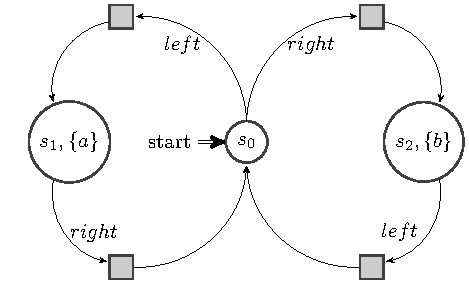
\includegraphics[width = 8cm]{reply_letter_MDP.pdf}
      \caption{The MDP with three states $s_0$, $s_1$, and $s_2$ and two actions $left$ and $right$. $s_1$ and $s_2$ are labeled with $\{ a \}$ and $\{ b \}$, respectively. The initial sate is $s_0$.}
      \label{MDP_counterexample}
  \end{figure}

  \begin{figure}[H]
     \centering
     \vspace{2mm}
  %   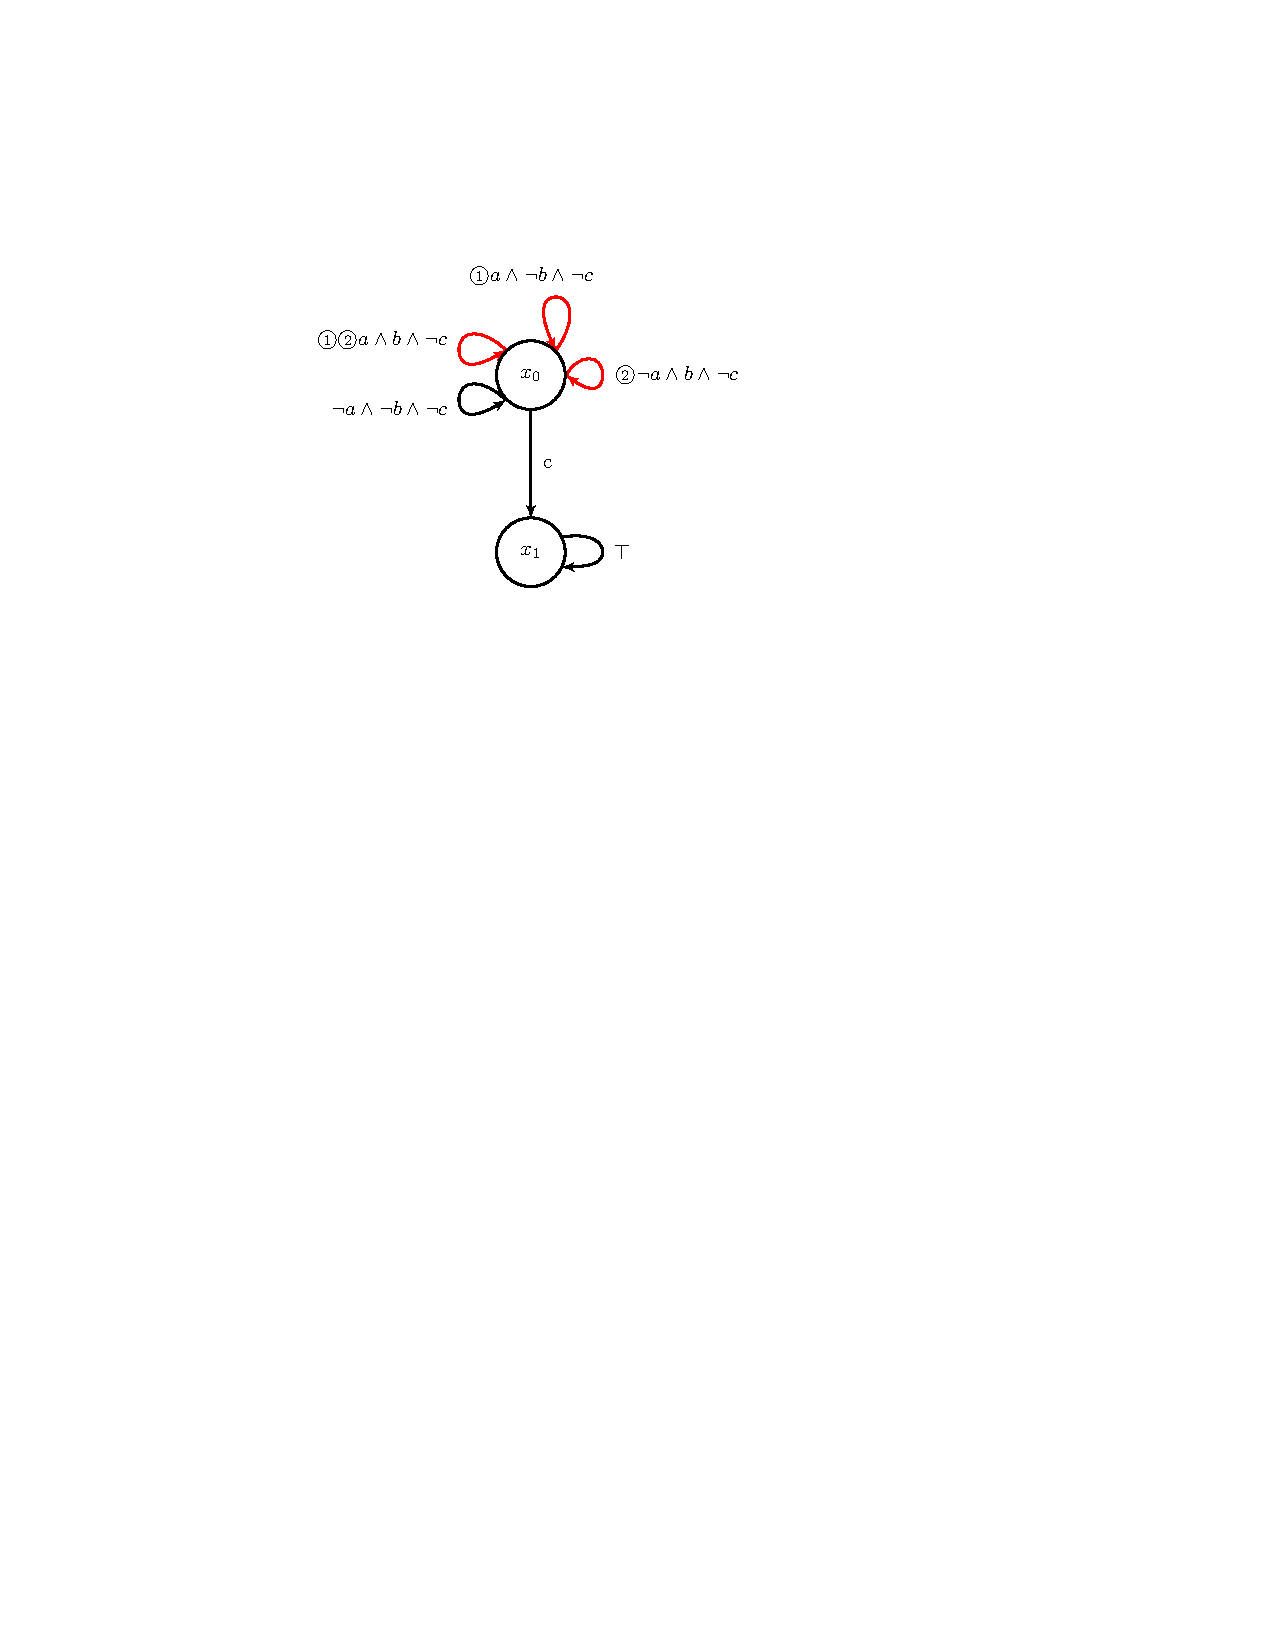
\includegraphics[bb=140 498 368 682,width=5cm]{automaton1.pdf}
     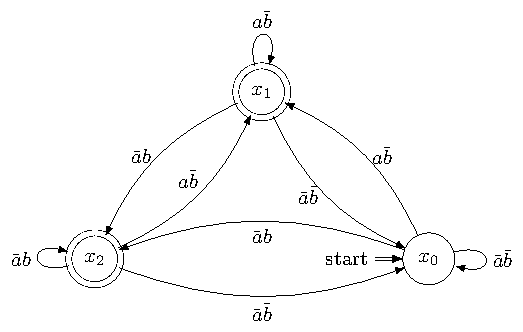
\includegraphics[width = 8cm]{reply_letter_LDBA.pdf}
     \caption{The state-based LDBA corresponding the LTL formula $\varphi = \text{{\bf GF}}a \land \text{{\bf GF}}b$. The accepting states are represented as double circles. The initial state is $x_0$.}
     \label{LDBA_counterexample}
  \end{figure}


\end{reply}

\begin{review point}
  The main benefit of using a LDBA is that its state space is smaller
than alternative automata such Rabin Automata. However, here due to
state augmentation (Definition 8) this advantage is lost. The authors
need to motivate the use of the LDBA in this paper and also report the
size of the state-space of the product MDP and compare it to [14]. The
latter is important for the scalability of the proposed algorithm.
\end{review point}

\begin{reply}
 As you pointed out, by the augmentation, the state space of an augmented tLDGBA corresponding to an LTL formula $\varphi$ is larger than a tLDBA corresponding to the same formula $\varphi$ and its size is about $\frac{2^{n}-1}{n}$ times, where $n$ is the number of all accepting sets of the original tLDGBA. We added a remark (Remark 1) explaining this point to our manuscript. The reason we use LDGBAs instead of other automata is mainly described in \cite{Hahn2019}. It is known that deterministic Rabin automata (DRA) and non-deterministic B\"{u}chi automata (NBA) can recognize all of the $\omega$-regular language. However, there is a counterexample of an MDP $M$ and an LTL formula $\varphi$ with Rabin index 2, which is mentioned in \cite{Hahn2019}, such that, although there is a positional policy satisfying $\varphi$ with probability 1 on $M^{\otimes}$ of $M$ and the DRA, any optimal policy obtained from any reward based on the acceptance condition of the DRA do not satisfy the LTL formula with probability 1. This is because the reward functions are defined for each acceptance pair of the acceptance condition of the DRA, namely the counterexample is due to that only one acceptance pair of the DRA is considered in one learning. Further, LDBAs are not only as expressive as NBAs but also the number of non-deterministic transitions are much less than NBAs.
\end{reply}

\begin{review point}
  Does maximizing the collection of the proposed rewards implies
maximization of the satisfaction probability? In other words, does the
proposed algorithm find a feasible or the optimal solution.
\end{review point}

\begin{reply}
 No, it is. It does not generally hold in our problem settings that maximizing expected discounted reward implies maximizing the satisfaction probability. We revised the conclusion in our manuscript to clarify that maximizing the satisfaction probability is one of future works.
\end{reply}

\begin{review point}
  The definition of the labeling function (page 2) is unusual. Typically, observations are assigned to states and not to transitions.
\end{review point}

\begin{reply}

\end{reply}

\begin{review point}
  In Definition 2, $last(\rho)$ is not defined anywhere in the text.
\end{review point}

\begin{reply}
  We defined $last(\rho)$ in the second paragraph of Definition 1.
\end{reply}

\section{Reply to Reviewer 7 (20009)}

\begin{review point}
  The probability function in Def. 9 can be not well-defined for
non-deterministic transitions. Consider a simple example, say $(x_1, l,
x_1')$ and $(x_1, l, x_2')$ are both in delta. $P(s'|s, a) =1$ with $l=
L((s,a,s'))$ will have two outgoing transitions labeled by the same
action a, and all with probability one. The sum of probability given
action a on state $(s, x_1)$ will be 2. Will this study only consider
deterministic transitions?
\end{review point}

\begin{reply}
  We added the explanation of $\varepsilon$-transitions in a tLDGBA to the definition of the limit-determinism. Then, we revised Definition 8 to clarify how we handle $\varepsilon$-transitions in an augmented tLDGBA.
\end{reply}

\begin{review point}
  The construction of augmented automaton in Def. 8 is not
well-motivated. What is the intuition behind this construction?
Further, there should be a formal proof that the two automata accepting
the same language. Examples in section IV helps a lot. It would be
useful to have a small example to illustrate the construction.
\end{review point}

\begin{reply}
  The intuition behind the construction is that we think the method in \cite{HAK2019} may not have a positional policy satisfying a given LTL formula on the corresponding product MDP.
  %there is an example of an MDP $M$ and an LTL formula $\varphi$ such that there exists no positional policy satisfying $\varphi$ on the product MDP of $M$ and the tLDGBA (or state-based LDGBA) corresponding to $\varphi$ if we use the reward function defined as the accepting frontier function \cite{HAK2019}.
  This is because that the original LDGBAs have less memory capacity than LDBAs and the accepting frontier function is memoryless. We believe it is expanded that the class of positional policies satisfying a given LTL formula on the corresponding product MDP by our augmentation. We added two remarks that explain the reason we used LDGBAs instead of other automata and that if we use original LDGBAs and the reward function defined as the accepting frontier function, there exists an example of an MDP $M$ and a given LTL formula $\varphi$ such that there exists no positional policy satisfying $\varphi$ on the product MDP of $M$ and a tLDGBA or a state-based LDGBA corresponding to $\varphi$. We have showed the example in section IV such that the method in \cite{HAK2019} cannot synthesize any positional policy satisfying the given LTL formula on the corresponding product MDP.

  Due to lack of space in our manuscript, we gave up to add the formal proof to the manuscript. So we proof the two automata accepts the same language only in the reply letter.

  \begin{theorem}
    A tLDGBA and its augmentation accept the same language.
  \end{theorem}

  \begin{proof}
    Let $B$ denote a tLDGBA and $\bar{B}$ denote its augmentation. Let a infinite input word $w$ be accepted by $B$ and $r$ be the infinite run of $B$ for $w$. Thus, $inf(r) \cap F_j \neq \emptyset$ holds for any accepting set $F_j$ of $B$, where $inf(r)$ is the set of transitions that occur infnitely often in the run $r$. In other words, the infinite accepting transitions of all accepting sets of $B$ are in $r$ regardless of its order. Then, we consider how the word $w$ is accepted by $\bar{B}$. By the definition of the acceptance condition of $\bar{B}$, two or more visits to an accepting set $F_j$ does not contribute to the acceptance by $\bar{B}$ until all accepting sets of $B$ are visited after the latest visits to them of $B$. For a current binary-valued vector $v$, if a current transition $(x,\sigma,x^{\prime})$ is in an accepting set $F_j$ that have been visited once or more after the latest visits to all accepting sets of $B$, $Max(v, visitf((x,\sigma,x^{\prime}))) = v$ holds. This is because the $j$-th element of $v$ is already 1 and $visitf((x,\sigma,x^{\prime}))$ returns a vector such that the $j$-th element is 1 and the rest of elements are 0. Therefore, by the definition of the acceptance condition of $\bar{B}$, the transition of $\bar{B}$ corresponding to $(x,\sigma,x^{\prime})$ is not in any accepting sets of $\bar{B}$.
    While, if the current transition $(x,\sigma,x^{\prime})$ is first visit to an accepting set $F_j$ of $B$ after the latest visits to all accepting sets of $B$, namely the $j$-th element of the current binary-valued vector is $0$, then $Max(v, visitf((x,\sigma,x^{\prime})))$ returns the vector such that the $j$-th element is 1 and the rest of elements are same as $v$. Therefore, by the definition of the acceptance condition of $\bar{B}$, the transition of $\bar{B}$ corresponding to $(x,\sigma,x^{\prime})$ is in the $j$-th accepting set $\bar{F}_j$ of $\bar{B}$.
    When all accepting sets of $B$ have visited at the transition $(\hat{x},\hat{\sigma},\hat{x}^{\prime})$, we have $Max(v, visitf(\hat{x},\hat{\sigma},\hat{x}^{\prime}))) = \bm{1}$ and $reset(Max(v, visitf((\hat{x},\hat{\sigma},\hat{x}^{\prime})))) = \bm{0}$. Subsequently, the same processing is performed on the run $r$, so that the input word $w$ is accepted by $\bar{B}$. Therefore, the language accepted by $B$ are also accepted by $\bar{B}$.

    Let $w^{\prime}$ denote the infinite input word accepted by $\bar{B}$ and $r^{\prime}$ be the infinite run of $\bar{B}$ for $w^{\prime}$. The run $r^{\prime}$ visits all accepting sets of $\bar{B}$ infinitely often. Thus, by the definition of the acceptance condition of $\bar{B}$, obviously the run in $X(\Sigma X)^{\omega}$ corresponding to $r^{\prime}$ visits all accepting sets of $B$ infinitely often. Therefore, the language accepted by $\bar{B}$ are also accepted by $B$.
  \end{proof}

  small example は論文の例題中のオートマトンで十分だと考えているのですがどうでしょうか.
\end{reply}

\begin{review point}
  In the proof of Lemma 1, the last sentence is unclear. The goal is to
show that either an agent receives no reward from visiting recurrent
class, or the agent has to visit all recurrent class for which the
acceptance condition are satisfied・ It is not clear why it is not
possible that a policy only visits some subset of acceptance set but
not all. This may due to the lack of explanation to the def.8.
\end{review point}

\begin{reply}
  We consider the unclarity of the proof of Lemma 1 is due to the lack of the explanation of Definition 8. So we added a statement with regard to the acceptance condition of an augmented automaton after its definition.
\end{reply}

\begin{review point}
  The construction of augmented automaton is similar to the accepting
frontier function in the following paper, presented at CDC this year: Hosein et
al.  mainly, the same problem was studied too. The authors should
highlight the difference and their unique contribution comparing to
existing work.
Reinforcement Learning for Temporal Logic Control Synthesis with
Probabilistic Satisfaction Guarantees
https://arxiv.org/pdf/1909.05304.pdf
\end{review point}

\begin{reply}
  We added a remark (Remark 2) to clarify the comparison between our proposed method and the method in \cite{HAK2019,HKAKPL2019}.
\end{reply}

\begin{review point}
  The comparison with [14] is unclear. If both methods generate the
optimal policies, then it is not clear why [14] does not perform
correctly in this example.
\end{review point}

\begin{reply}
  We revised the statement of the results. The result for the method in \cite{HAK2019} is due to that it is impossible the transitions labeled by $\{ a \}$ and $\{ b \}$ occur from $s_4$ infinitely often by any positional policy with the tLDBA. In detail, the state of the tLDBA is always $x_0$ while the agent does not move to states $s_2$, $s_3$, $s_5$, and $s_6$. Thus, the state of the product MDP is always $(s_4, x_0)$ while the agent stays in $s_4$. While our proposed method can recognize the previous visits as a state. Thus, our proposed method can synthesize a positional policy satisfying $\varphi$ on the product MDP, while the method in \cite{HAK2019} cannot. Therefore, the method in \cite{HAK2019} may not synthesize positional policies satisfying LTL specifications on the product MDP depending on the settings of MDPs or LTL specifications.
\end{reply}

\begin{review point}
  The notations are too complicated and can be simplified.
\end{review point}

\begin{reply}

\end{reply}

\begin{review point}
  Def. 7 is bit complicated in writing, the definition in ref.[13] is
much clearer. Further, the statement the transitions in each part are
deterministic・・this claim is not suggested in [13]. In fact, in the
original definition, the state space partitions to the nondeterministic
part and deterministic part. The transitions in the nondeterministic
part can be nondeterministic.
\end{review point}

\begin{reply}
  We revised the definition of limit-determinism and employed the definition like \cite{SEJK2016}. Then, we explain that the transitions in initial part are deterministic because of its construction.
\end{reply}

\section{Reply to Reviewer 8 (20011)}

\begin{review point}
  The paper is well-written and organized well. There are lot of
symbols with subscripts, superscripts in the paper and it might be
helpful to include a paragraph that describes the notation.
\end{review point}

\begin{reply}

\end{reply}

\begin{review point}
  How is the reward function defined in the example for the method in
\cite{HAK2019}? Can the two rewards be compared?
\end{review point}

\begin{reply}
  We defined the reward function in the example for the method in \cite{HAK2019} as the accepting frontier function defined in \cite{HAK2019} and the immediate reward is the same value as the reward for our proposed method. If an optimal policy on the product MDP were satisfying the LTL formula $\varphi$, the agent could visit $s_0$, $s_8$ infinitely often and would never visit $s_2$, $s_3$, $s_5$, and $s_6$, and would accumulate rewards just like the agent under the our proposed method. Therefore, the two rewards can be compared.
\end{reply}

\begin{review point}
  How does the proposed method compare in terms of computational
complexity with other methods? This would be helpful information for
the readers especially since the proposed method depends on augmenting
the LDBA.
\end{review point}

\begin{reply}
  We interpret the computational complexity as the size of the state space of an automaton. In general, when constructing a transition-based B\"{u}chi automaton (tBA) from a transition-based generalized B\"{u}chi automaton (tGBA), the order of visits to accepting sets of the tGBA is fixed. Consequently, the reward based on the acceptance condition of the tBA tends to be sparse and the sparsity is critical against RL-based control policy synthesis problems. The augmentation of tGBA relaxes the sparsity since the augmented tGBA has all of the order of visits to all accepting sets of the original tGBA. The size of the state space of the augmented tGBA is about $\frac{2^{n}-1}{n}$ times larger than the tBA, however, the ratio of the number of accepting transitions to the number of all transitions of the augmented tGBA is much greater than the tBA.
\end{reply}

\begin{thebibliography}{99}
\bibitem{Hahn2019}
E.\ M.\ Hahn, M.\ Perez, S.\ Schewe, F.\ Somenzi, A.\ Triverdi, and D.\ Wojtczak,
``Omega-regular objective in model-free reinforcement learning,''
\textit{Lecture Notes in Computer Science}, no.\ 11427, pp.\ 395--412, 2019.
\bibitem{HAK2019}
M.\ Hasanbeig, A.\ Abate, and D.\ Kroening,
``Logically-constrained reinforcement learning,'' \textit{arXiv:1801.08099v8}, Feb.\ 2019.
\bibitem{HKAKPL2019}
M.\ Hasanbeig, Y.\ Kantaros, A.\ Abate, D.\ Kroening, G.\ J.\ Pappas, and I.\ Lee,
``Reinforcement learning for temporal logic control synthesis with probabilistic satisfaction guarantee,''
\textit{arXiv:1909.05304v1}, 2019.
\bibitem{BWZP2019}
A.\ K.\ Bozkurt, Y.\ Wang, M.\ Zavlanos, and M.\ Pajic,
``Control synthesis from linear temporal logic specifications using model-free reinforcement learning,''
\textit{arXiv:1909.07299}, 2019.
\bibitem{SEJK2016}
S.\ Sickert, J.\ Esparaza, S.\ Jaax, and J.\ K\v{r}et\`{i}nsk\'{y},
``Limit-deterministic B\"{u}chi automata for linear temporal logic,''
 in \textit{International Conference on Computer Aided Verification}, 2016, pp.\ 312-332.
\end{thebibliography}

\end{document}
